%; whizzy chapter
% -initex iniptex -latex platex -format platex -bibtex jbibtex -fmt fmt
% $B0J>e(B whizzytex $B$r;HMQ$9$k>l9g$N@_Dj!#(B

%     Kansai Debian Meeting resources
%     Copyright (C) 2007 Takaya Yamashita
%     Thank you for Tokyo Debian Meeting resources

%     This program is free software; you can redistribute it and/or modify
%     it under the terms of the GNU General Public License as published by
%     the Free Software Foundation; either version 2 of the License, or
%     (at your option) any later version.

%     This program is distributed in the hope that it will be useful,
%     but WITHOUT ANY WARRANTY; without even the implied warranty of
%     MERCHANTABILITY or FITNESS FOR A PARTICULAR PURPOSE.  See the
%     GNU General Public License for more details.

%     You should have received a copy of the GNU General Public License
%     along with this program; if not, write to the Free Software
%     Foundation, Inc., 51 Franklin St, Fifth Floor, Boston, MA  02110-1301 USA

%  preview (shell-command (concat "evince " (replace-regexp-in-string "tex$" "pdf"(buffer-file-name)) "&"))
% $B2hA|%U%!%$%k$r=hM}$9$k$?$a$K$O(Bebb$B$rMxMQ$7$F(Bboundingbox$B$r:n@.!#(B
%(shell-command "cd image200708; ebb *.png")

%%$B$3$3$+$i%X%C%@3+;O!#(B

\documentclass[mingoth,a4paper]{jsarticle}
\usepackage{kansaimonthlyreport}
\usepackage[dvips]{xy}

% $BF|IU$rDj5A$9$k!"Kh7nJQ$o$j$^$9!#(B
\newcommand{\debmtgyear}{2009}
\newcommand{\debmtgdate}{25}
\newcommand{\debmtgmonth}{10}
\newcommand{\debmtgnumber}{28}

\begin{document}

\begin{titlepage}

% $BKh7nJQ99$9$kItJ,!"K\J8$NKvHx$b=$@5$9$k$3$H$r$o$9$l$:$K(B

 $BBh(B\debmtgnumber{}$B2s(B $B4X@>(B Debian $BJY6/2q;qNA(B

\vspace{2cm}

\begin{center}
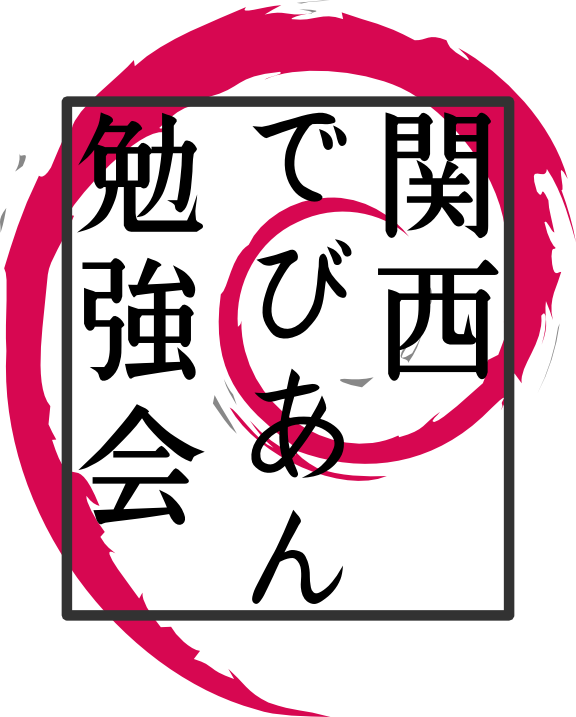
\includegraphics{image200802/kansaidebianlogo.png}
\end{center}

\begin{flushright}
\hfill{}$B4X@>(B Debian $BJY6/2qC4Ev<T(B $B:4!9LZ!&ARI_!&$N$,$?(B\\
\hfill{}\debmtgyear{}$BG/(B\debmtgmonth{}$B7n(B\debmtgdate{}$BF|(B
\end{flushright}

\thispagestyle{empty}
\end{titlepage}

\dancersection{Introduction}{Debian JP}

 $B4X@>(B Debian $BJY6/2q$O(BDebian GNU/Linux $B$N$5$^$6(B
 $B$^$J%H%T%C%/(B($B?7$7$$%Q%C%1!<%8!"(BDebian $BFCM-$N5!G=$N;EAH!"(BDebian $B3&7($G5/(B
 $B$3$C$?=PMh;v!"$J$I$J$I!K$K$D$$$FOC$79g$&2q$G$9!#(B

 $BL\E*$H$7$F<!$N;0$D$r9M$($F$$$^$9!#(B
 \begin{itemize}
  \item ML$B$d7G<(HD$G$O$J$/!"D>@\4i$r9g$o$;$k;v$G$N>pJs8r49$NB%?J(B
  \item $BDj4|E*$K=8$^$l$k>l=j(B
  \item $B;qNA$N:n@.(B
 \end{itemize}

 $B$=$l$G$O!"3Z$7$$$R$H$H$-$r$*2a$4$72<$5$$!#(B

\newpage

\begin{minipage}[b]{0.2\hsize}
 {\rotatebox{90}{\fontsize{80}{80}
{\gt $B4X@>%G%S%"%sJY6/2q(B}}}
\end{minipage}
\begin{minipage}[b]{0.8\hsize}
\hrule
\vspace{2mm}
\hrule
\setcounter{tocdepth}{1}
\tableofcontents
\vspace{2mm}
\hrule
\end{minipage}

%-------------------------------
\dancersection{$B:G6a$N(B Debian $B4X78$N%$%Y%s%HJs9p(B}{Debian JP}

\subsection{$BA02s$N4X@>(B Debian $BJY6/2q(B}

$BA02s$N4X@>(BDebian$BJY6/2q$O!"(B9$B7n(B27$BF|$K5~ET%j%5!<%A%Q!<%/$K$F3+:E$5$l$^$7$?!#(B

$B4X@>(BDebian$BJY6/2q=i$N5~ET$G$N3+:E$G$7$?$,!"=i;22C$NJ}$bB?$/;22C$5$l!"<+8J(B
$B>R2p$G$O%i%$%H%K%s%0%H!<%/$r$5$l$kJ}$bB3=P$7$F!"$+$J$j@9$j>e$,$j$^$7$?!#(B

$BH/I=$O!"$N$,$?$8$e$s$5$s$K$h$k(B reportbug$B$r;H$C$F(BDebian$B$N%P%0Js9p$r$*$3$J(B
$B$&J}K!$N2r@b!V(BGUI$B$,$D$$$F$+$C$3$h$/$J$C$?(Breportbug$B$r;H$C$F$_$h$&!W$H!":4!9(B
$BLZMNJ?$5$s$K$h$k(Bdebian.mentors.org$B$rMxMQ$7$F!"(BDebian$B%Q%C%1!<%8$r8x<0%j%](B
$B%8%H%j$K<h$j9~$s$G$b$i$&$?$a$NN.$l$r2r@b$7$?!V(Bdebian mentors$B$C$F$4B8CN$G(B
$B$9$+(B?$B!W$G$7$?!#(B

Debian$B$N%P%0Js9p$NJ}K!$d!"<+:n%Q%C%1!<%8$r8x<0%j%]%8%H%j$K<h$j9~$s$G$b$i(B
$B$&$?$a$NN.$l$,$h$/$o$+$j!"$H$F$b$h$+$C$?$N$G$O$J$$$G$7$g$&$+!#(B

\begin{figure}[h]
 \begin{center}
 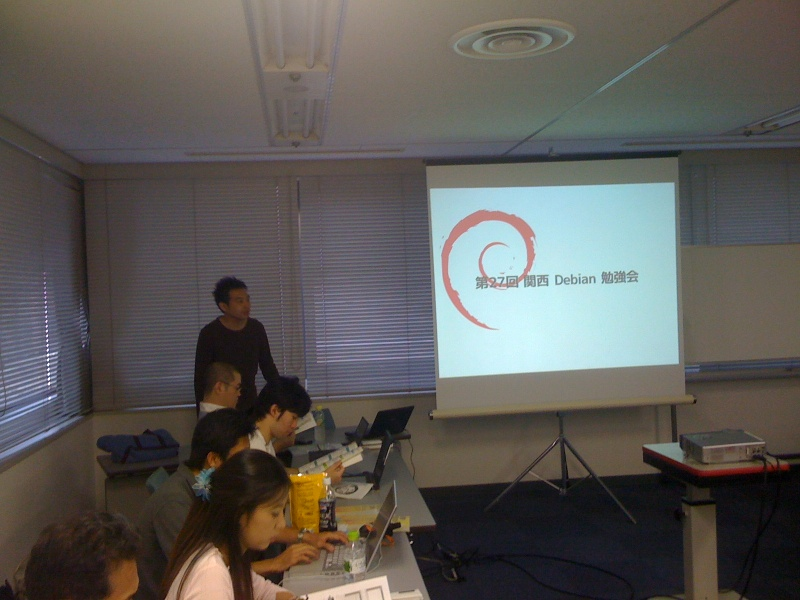
\includegraphics[width=6cm]{image200910/kyoto01.jpg}
 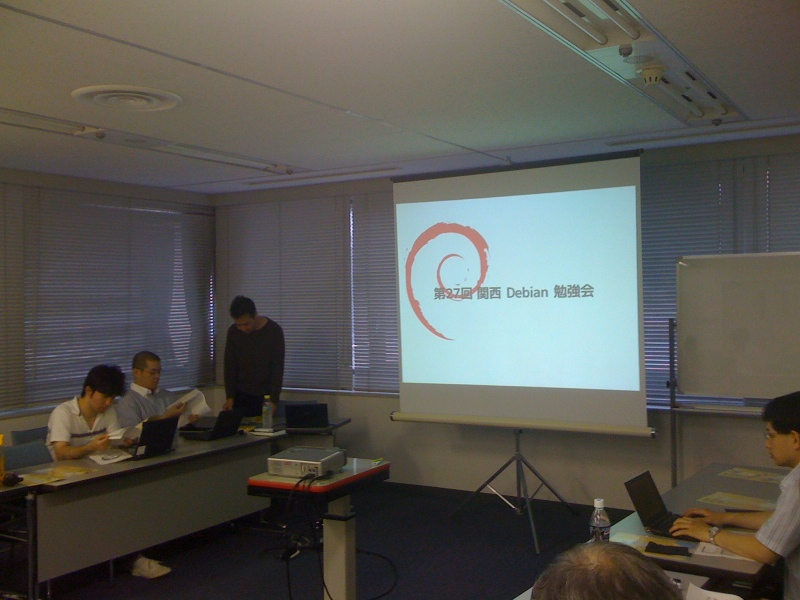
\includegraphics[width=6cm]{image200910/kyoto02.jpg}
 \caption{$B5~ET$G$NJY6/2q$NMM;R(B}
 \end{center}
\end{figure}


%-------------------------------
\dancersection{$B%G%P%C%0$N$*6!!'(B"gdb$B$N%9%9%a(B"}{$B?yK\E5=<(B}

\makeatletter
   \renewcommand{\thetable}{%
   \thesection.\arabic{table}}
   \@addtoreset{table}{section}
\makeatother

\makeatletter
    \renewcommand{\thefigure}{%
    \thesection.\arabic{figure}}
    \@addtoreset{figure}{section}
\makeatother


\subsection{$B$O$8$a$K(B}
$B%$%s%?!<%M%C%H$G$OMM!9$J%*!<%W%s%=!<%9$N%W%m%0%i%`$,8x3+$5$l$F$$$^$9!#$=$l$i$N%W%m%0%i%`$O3+H/<T$N<j$K$h$k%G%P%C%0$@$1$G$J$/!"B?$/$N?M$b%G%P%C%0:n6H$K;22h$9$k$3$H$K$h$C$FIJ<A$r9b$a$F$$$-$^$9!#$=$N%G%P%C%0:n6H$r=*$($?%W%m%0%i%`$,$$$o$f$k!V0BDj$7$?%W%m%0%i%`!W$G$"$j!"B?$/$N?M$,0B?4$7$F;H$($k%l%Y%k$K$J$k$K$O%G%P%C%0:n6H$O$H$F$bBg@Z$J:n6H$N(B1$B$D$G$9!#(B
$B:#2s$O!"(BDebian$B$r;H$C$F%W%m%0%i%`$r%G%P%C%0$9$k<jK!$K$D$$$F$^$H$a$F$_$^$7$?!#(B

\subsection{gdb$B$H$O(B}
gdb$B$H$O(BGNU Debugger\footnote{GNU Debugger Web$B%5%$%H(B
\url{http://www.gnu.org/software/gdb/}}$B$N$3$H$G!"(BC$B8@8l!&(BC++$B8~$1$N%=!<%9%l%Y%k%G%P%C%,$G$9!#3+H/<T$O(Bgdb$B$r;H$&$3$H$G%W%m%0%i%`$,:#$I$3$NItJ,$r<B9T$7$F$$$k$+!"%W%m%0%i%`$N>uBV$O$I$&$J$C$F$$$k$+$rCN$k$3$H$,$G$-$k$?$a!"%G%P%C%0:n6H$r8zN(E*$K9T$&$3$H$,$G$-$^$9!#(B
$B!V(Bman gdb(1)$B!W$K$h$k$H!"(Bgdb$B$K$OBg$-$/(B4$B$D$N5!G=$,$"$k$H=q$+$l$F$$$^$9!#(B
\begin{itemize}
 \item $B%W%m%0%i%`$NF0:n$r>\:Y$K;XDj$7$F%W%m%0%i%`$r<B9T$5$;$k!#(B
 \item $B;XDj$7$?>r7o$G%W%m%0%i%`$rDd;_$5$;$k!#(B
 \item $B%W%m%0%i%`$,;_$^$C$?;~$K!"2?$,5/$3$C$?$+D4$Y$k!#(B
 \item $B%P%0$K$h$kI{:nMQ$r=$@5$7!"JL$N%P%0$rD4$Y$k$?$a%W%m%0%i%`$N>uBV$rJQ99$9$k!#(B
\end{itemize}

gdb$B$,;HMQ$9$k@_Dj%U%!%$%k$O(B"$B!A(B/.gdbinit"$B$G$"$j!"(Bgdb$B$N=i4|@_DjCM$r$3$N%U%!%$%k$KDj5A$9$k$3$H$GJQ99$G$-$^$9!#(B

\subsection{$B3+H/4D6-$H(Bgdb$B$N%$%s%9%H!<%k(B}
C$B8@8l$N%W%m%0%i%`$r3+H/$9$k$?$a$K$O%3%s%Q%$%i$,I,MW$G$9!#(Bgdb$B$NB>$K%W%m%0%i%`$r:n@.$9$k$?$a$KI,MW$J%=%U%H%&%'%"0l<0$b%$%s%9%H!<%k$7$^$9!#(B
\begin{commandline}
$ sudo apt-get update
$ sudo apt-get install gcc make
$ sudo apt-get install gdb
\end{commandline}

$B4D6-$b@0$C$?$H$3$m$G!"%W%m%0%i%`$r:n@.$7$^$9!#:#2s$O!V(BFizzBuzz$B!W(B\footnote{FizzBuzz$B$H$O!"!X(B1$B$+$i(B100$B$+$i$^$G$N@0?t$rI8=`=PNO$K=PNO$;$h!#$?$@$7!"(B3$B$G3d$j@Z$l$k$H$-$O!V(BFizz$B!W!"(B5$B$G3d$j@Z$l$k$H$-$O!V(BBuzz$B!W!"(B3$B$H(B5$B$NN>J}$G3d$j@Z$l$k$H$-$O!V(BFizzBuzz$B!W$HI8=`=PNO$K=PNO$;$h!#!Y$H$$$&%W%m%0%i%`$NLdBj$G$"$k!#(B}$B$H$$$o$l$F$$$k%W%m%0%i%`$rNc$K$7$F$_$^$9!#(B

\subsection{gdb$B$r;H$C$F$_$^$7$g$&(B}
\subsubsection{$B$^$:$O%G%P%C%0%S%k%I$7$^$9(B}
$B%W%m%0%i%`$r(Bgdb$B$GA`:n$9$k$?$a$K$O%W%m%0%i%`$K%G%P%C%0>pJs$rIUM?$7$F%S%k%I$9$kI,MW$,$"$j$^$9!#(B
gcc$B$N%3%s%Q%$%k%*%W%7%g%s5Z$S%S%k%I%*%W%7%g%s$K%G%P%C%0%7%s%\%k$rIUM?$9$k(B"-g"$B%*%W%7%g%s$r$D$1$F%S%k%I$7$^$9!#!J%G%P%C%0;~$N:GE,2=%l%Y%k$O3+H/<T$K$h$C$F;XDj$,0c$&$3$H$b$"$j$^$9!#$3$3$G$O:GE,2=%l%Y%k$OL5;XDj(B(="-O0"$B!":GE,2=$J$7(B)$B$H$7$F%S%k%I$7$^$9!#!K(B


\subsubsection{gdb$BC1BN$G%W%m%0%i%`$rDI$$$+$1$F$_$k(B}
$B$=$l$G$O%7%'%k$+$i(Bgdb$B$r5/F0$7$^$9!#(Bgdb$B$r5/F0$9$k$H0J2<$N$h$&$JF~NO<uIU>uBV$K$J$j$^$9!#(B

\begin{commandline}
$ gdb
GNU gdb 6.8-debian
Copyright (C) 2008 Free Software Foundation, Inc.
License GPLv3+: GNU GPL version 3 or later <http://gnu.org/licenses/gpl.html>
This is free software: you are free to change and redistribute it.
There is NO WARRANTY, to the extent permitted by law.  Type "show copying"
and "show warranty" for details.
This GDB was configured as "x86_64-linux-gnu".
(gdb) 
\end{commandline}

gdb$B$N%W%m%s%W%H$G%3%^%s%I$rF~NO$9$k$3$H$K$h$j%G%P%C%,$rDL$7$F%W%m%0%i%`$rF0$+$9$3$H$,$G$-$^$9!#(B
$B%G%P%C%0:n6H$G$h$/;H$&(Bgdb$B$N%3%^%s%I$rI=(B\ref{table_use_gdb}$B$K<($7$^$9!#(B

\begin{table}[h]
\begin{center}
\caption{gdb$B$rA`:n$9$k%3%^%s%I(B($B0lItH4?h(B)}\label{table_use_gdb}
\begin{tabular}{|l|c|p{9cm}|}
\hline
$B%3%^%s%I(B & $B>JN,%3%^%s%I(B & $B@bL@(B \\ \hline \hline
run ($B0z?t(B)& r & $B%W%m%0%i%`$r:G=i$+$i<B9T$7$^$9!#(B\\
 & & $B0z?t$r;XDj$9$k>l9g$O!"(Brun$B$N8e$K0z?t$r;XDj$7$^$9!#(B \\ \hline
break ($BDd;_0LCV(B) & b & $B%V%l!<%/%]%$%s%H$r@_Dj$7$^$9!#%V%l!<%/%]%$%s%H$O!V4X?tL>!W$H!V%=!<%9%3!<%I(B:$B9THV9f!W$N$$$:$l$+$G;XDj$G$-$^$9!#(B\\ \hline
delete (breakpoint$BHV9f(B)& d & $B%V%l!<%/%]%$%s%H$r:o=|$7$^$9!#C1$K(Bdelete$B$@$1$r<B9T$9$k$H$9$Y$F$N%V%l!<%/%]%$%s%H$r:o=|$7$^$9!#(B\\ \hline
list & l & $B8=:_<B9TCf$N6a$/$N%=!<%9%3!<%I$r$"$k9T?tI=<($7$^$9!#(B($B=i4|@_DjCM$O(B10$B9T(B)\\ \hline
step & s & $B%9%F%C%W%$%s<B9T$7$^$9!#(B\\ \hline
next & n & $B%9%F%C%W%*!<%P!<<B9T$7$^$9!#(B\\ \hline
finish & fin & $B%9%F%C%W%"%&%H<B9T$7$^$9!#(B\\ \hline
continue & c & $B8=:_Dd;_Cf$N0LCV$+$i%W%m%0%i%`$r:F3+$7$^$9!#(B\\ \hline
print ($BJQ?tL>(B) & p & $B%W%m%0%i%`Cf$N(B($BJQ?tL>(B)$B$NFbMF$rI=<($7$^$9!#%]%$%s%?JQ?t$N>l9g$O!V(Bprint *$B%]%$%s%?JQ?tL>!W$H;XDj$9$k$3$H$G%]%$%s%H$,;X$7<($9CM$rI=<($G$-$^$9!#(B\\ \hline
set var ($BJQ?tL>(B)=($B@_DjCM(B) & $B$J$7(B & $B%W%m%0%i%`Cf$N(B($BJQ?tL>(B)$B$NCM$r(B($B@_DjCM(B)$B$KJQ99$7$^$9!#(B\\ \hline
quit & q & gdb$B$r=*N;$7$^$9!#(B\\ \hline
attach ($B%W%m%;%9(BID)& $B$J$7(B & $B<B9TCf$N(B($B%W%m%;%9(BID)$B$r(Bgdb$B$G@)8f$G$-$k$h$&$K$7$^$9!#(B\\ \hline
detach & $B$J$7(B & attach$BCf$N%W%m%;%9$r(Bgdb$B$N@)8f2<$+$i@Z$jN%$7$^$9!#@Z$jN%$5$l$?%W%m%0%i%`$O$=$N$^$^F0:n$7B3$1$^$9!#(B\\ \hline
shell & $B$J$7(B & shell$B$r5/F0$7$^$9!#(Bshell$B$r(Bexit$B$9$k$H(Bgdb$B%W%m%s%W%H$KLa$j$^$9!#(B\\ \hline
help & h & gdb$B$N%3%^%s%I$K4X$9$k%X%k%W$rI=<($7$^$9!#(B\\ \hline
info ($B%3%^%s%I(B) & i & $BMM!9$J>pJs$rI=<($7$^$9!#(B\\ \hline
\end{tabular}
\end{center}
\end{table}

\subsection{gdb$B$N%U%m%s%H%(%s%I%D!<%k(B}
gdb$B$OC1BN$G$b==J,%G%P%C%02DG=$G$9$,!"$h$j%G%P%C%0:n6H$r9T$$$d$9$$$h$&$K(Bgdb$B$N%U%m%s%H%(%s%I%D!<%k$,B?$/$"$j$^$9!#(B
X Window System$B>e$GF0:n$9$kE}9g3+H/4D6-(B(IDE)$B$G$O(BKDevelop$B!"(BAnjuta$B!"(BEclipse$B!"(BNetBeans$B$J$I!"%3%^%s%I%i%$%s>e$G$bF0:n$9$k(BEmacs$B!"(BVim$B$J$I$b%U%m%s%H%(%s%I$H$7$FMxMQ$9$k$3$H$,$G$-$^$9!#(B

\subsubsection{Emacs GUD$B%b!<%I$G(Bgdb$B$r;H$C$F$_$k(B}
Emacs$B$K$O(BGUD(Grand Unified Debugger)$B$H$$$&5!G=$,$"$j!"(BEmacs$B>e$GMM!9$J%G%P%C%,$HO"7H$9$k$3$H$,$G$-$k;EAH$_$G$9!#(BGUD$B$O(Bgdb$B$K8B$i$:!"(Bperldb(perl$BMQ%G%P%C%,(B)$B$d(Bpdb(python$BMQ%G%P%C%,(B)$B$J$I$b5/F0$9$k$3$H$,$G$-$^$9!#(B

Emacs$B$N<B9TCf$K0J2<$N%-!<$rF~NO$7$F(Bgdb$B$r5/F0$7$^$9!#(B

\begin{commandline}
M-x gdb
\end{commandline}

$B$=$N8e!"%_%K%P%C%U%!$G<B9T%U%!%$%k$r;XDj$7$F(BEnter$B%-!<$rF~NO$7$^$9!#(B

\begin{commandline}
Run gdb (like this): gdb --annotate=3 ../a.out
\end{commandline}

$B$9$k$H?^(B\ref{figure-emacs-gud1}$B!"?^(B\ref{figure-emacs-debugging1}$B$N$h$&$J2hLL$K@Z$jBX$o$j$^$9!#(B

\begin{figure}[H]
\begin{center}
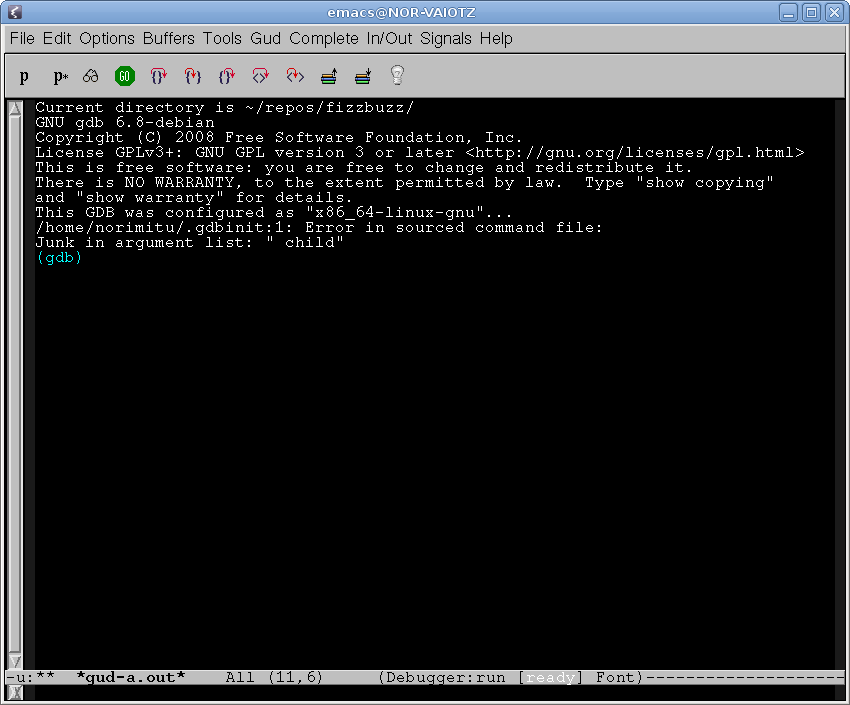
\includegraphics[scale=0.5]{image200910/gdb-emacs-gud1.png}
\caption{Emacs GUD$B%b!<%I$G(Bgdb$B$r5/F0$7$?2hLL(B(1)}\label{figure-emacs-gud1}
\end{center}
\end{figure}

\begin{figure}[H]
\begin{center}
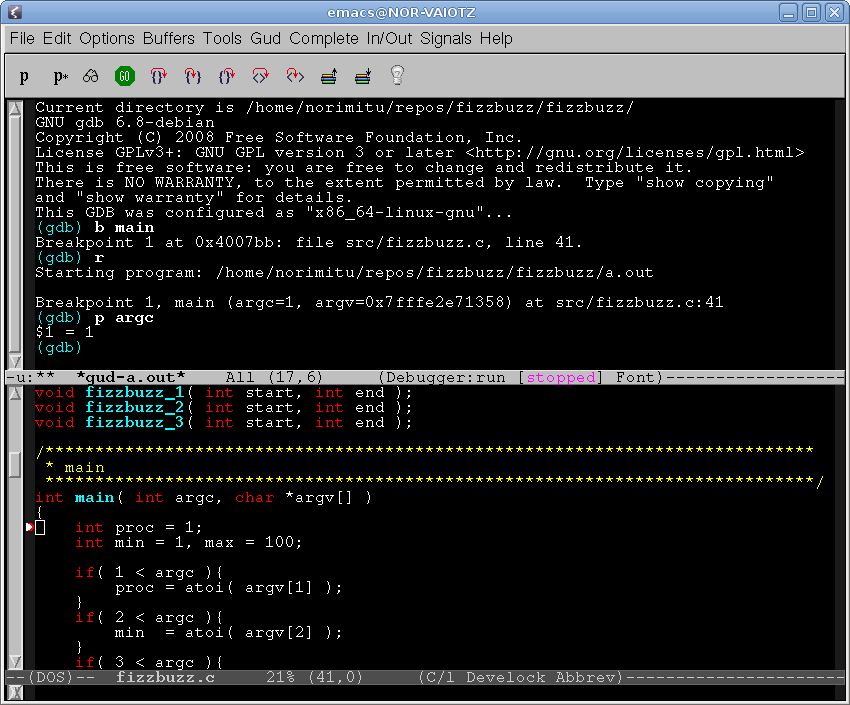
\includegraphics[scale=0.5]{image200910/gdb-emacs-gud2.png}
\caption{Emacs GUD$B%b!<%I$G%G%P%C%0Cf$N2hLL(B(2)}\label{figure-emacs-debugging1}
\end{center}
\end{figure}


$B$^$?!"(BEmacs$B$N@_Dj%U%!%$%k(B"$B!A(B/.emacs.el"$B$K!V(B(setq gdb-many-windows t)$B!W$r;XDj$7$F$*$/$H!"$9$k$H?^(B\ref{figure-emacs-gud2}$B!"?^(B\ref{figure-emacs-debugging2}$B$N$h$&$J2hLL$G(Bgdb$B$,5/F0$7$^$9!#(B
$B$3$N2hLL$rI=<($9$k$K$O!V(Bgud.el$B!W$H$$$&%U%!%$%k$,I,MW$G$"$j!#(Blenny$B$N>l9g$O(BEmacs$B$r%$%s%9%H!<%k$9$k$H0l=o$K%$%s%9%H!<%k$5$l$^$9!#(B

\begin{figure}[H]
\begin{center}
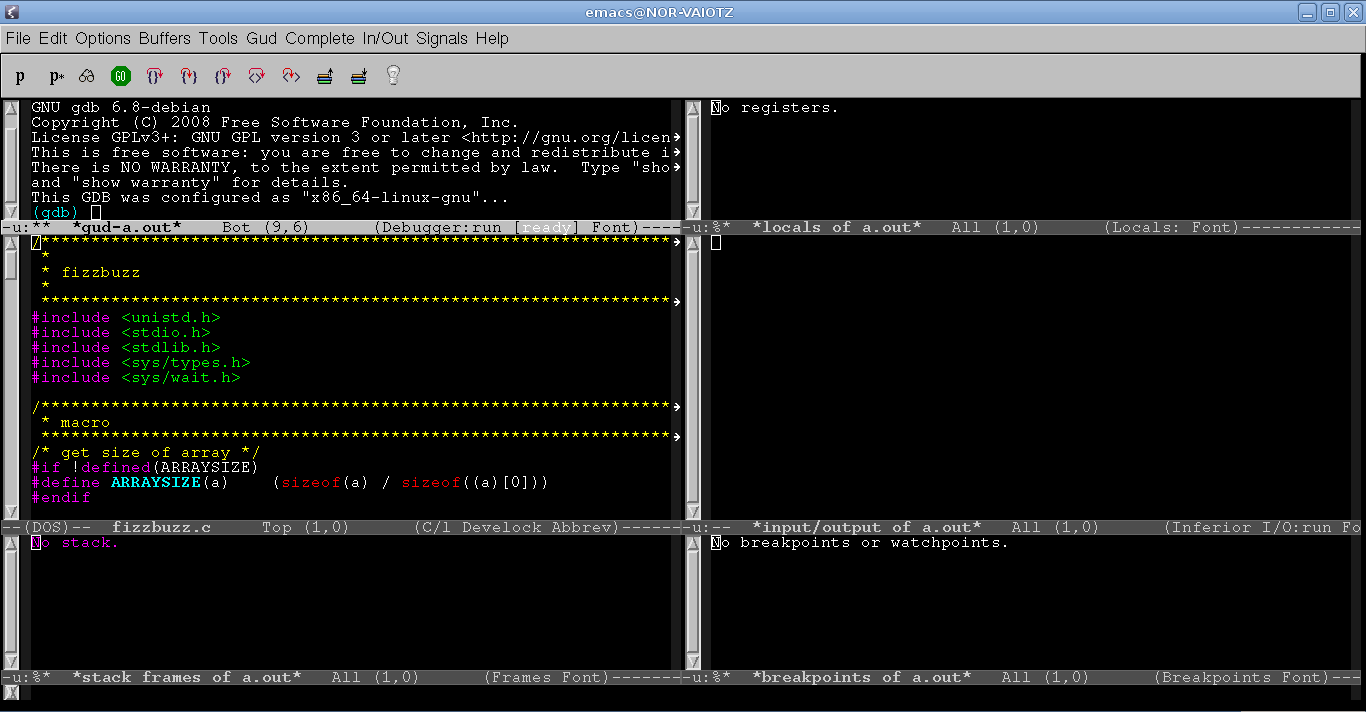
\includegraphics[scale=0.5]{image200910/gdb-emacs-gud3.png}
\caption{Emacs GUD$B%b!<%I$G(Bgdb$B$r5/F0$7$?2hLL(B(3)}\label{figure-emacs-gud2}
\end{center}
\end{figure}

\begin{figure}[H]
\begin{center}
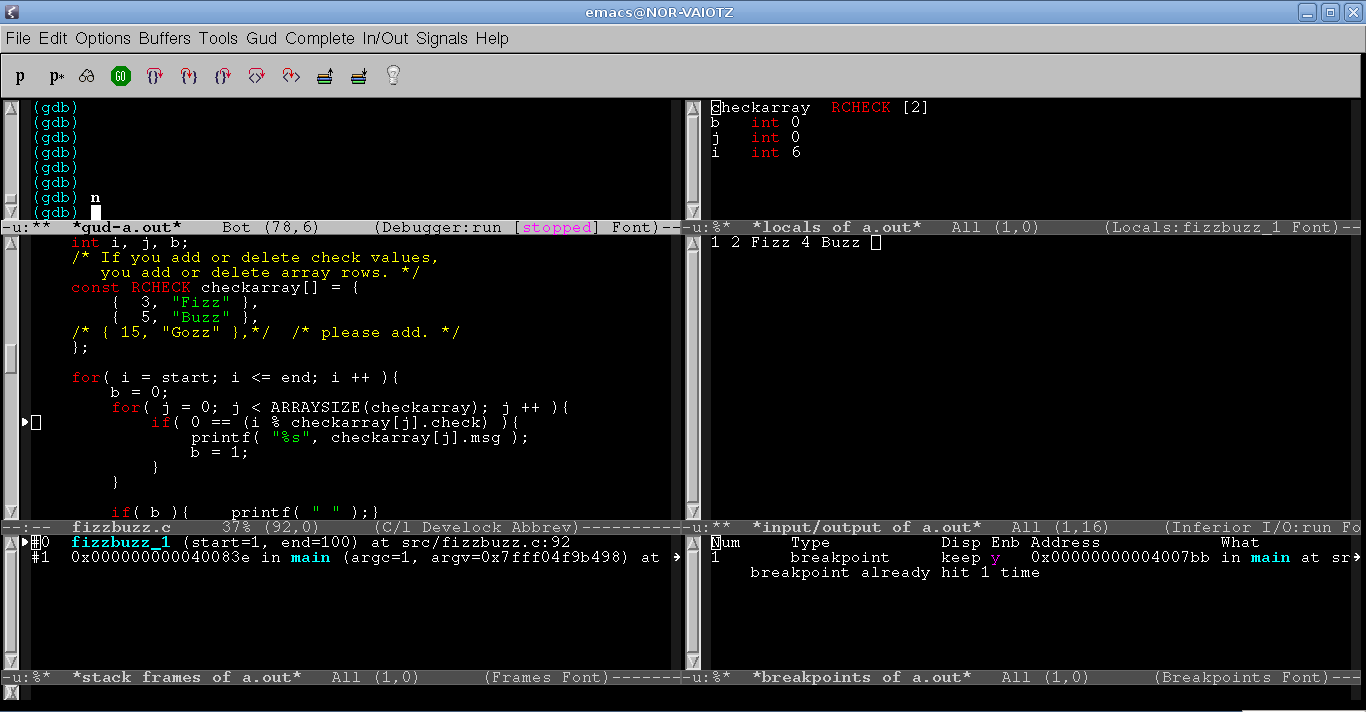
\includegraphics[scale=0.5]{image200910/gdb-emacs-gud4.png}
\caption{Emacs GUD$B%b!<%I$G%G%P%C%0Cf$N2hLL(B(4)}\label{figure-emacs-debugging2}
\end{center}
\end{figure}


\subsection{$B$$$m$$$m$J%W%m%0%i%`$N%G%P%C%0J}K!(B}
$B;d$,%W%m%0%i%`$r(Bgdb$B$r;H$C$F%G%P%C%0$9$k$H$-$NA`:nNc$r5s$2$F$_$^$9!#(B

\subsubsection{$BC1H/<B9T7O%W%m%0%i%`$N%G%P%C%0(B}
$BC1H/<B9T$9$k%W%m%0%i%`$N>l9g$O%G%P%C%,$G%W%m%0%i%`$N5/F0$r9T$$!"$=$N8e$K%G%P%C%0:n6H$r3+;O$9$k$3$H$K$J$j$^$9!#(B

\begin{enumerate}
\item gdb$B$r5/F0$7$^$9!#(B
\item break$B%3%^%s%I$G%V%l!<%/%]%$%s%H$r;XDj$7$^$9!#(B($B<B:]$K$O!V(Bb main$B!W$HF~NO$7$F%W%m%0%i%`$N:G=i$G;_$a$k$3$H$bB?$$$G$9!#(B)
\item run$B%3%^%s%I$G%W%m%0%i%`$r3+;O$7$^$9!#(B
\item step$B%3%^%s%I!"(Bnext$B%3%^%s%I$G%W%m%0%i%`$rDI$$$+$1$^$9!#(B
\item $B%G%P%C%0$,40N;$7$?$i!"(Bcontinue$B%3%^%s%I$G;D$j$N%W%m%0%i%`$9$Y$F$r<B9T$7$^$9!#(B
\item quit$B%3%^%s%I$G(Bgdb$B$r=*N;$7$^$9!#(B
\end{enumerate}

\subsubsection{$B%G!<%b%s7O%W%m%0%i%`$N%G%P%C%0(B}
$B%G!<%b%s$H$7$FF0:n$7$F$$$k%W%m%0%i%`$N>l9g$O!"F0:nCf$N%W%m%0%i%`$r(Bgdb$B$G@)8f$9$kI,MW$,$"$k$?$a%"%?%C%A$9$kI,MW$,$"$j$^$9!#(B

\begin{enumerate}
\item $B%G%P%C%0$9$k%G!<%b%s%W%m%0%i%`$r<B9T$7$^$9!#(B
\item $B%G%P%C%0$9$k%G!<%b%s%W%m%;%9$N%W%m%;%9(BID$B$rD4$Y$^$9!#(B
\item gdb$B$r5/F0$7$^$9!#(B
\item $B%W%m%;%9(BID$B$r;XDj$7$F(Battach$B%3%^%s%I$r<B9T$7!"%G%P%C%0$9$k%G!<%b%s%W%m%;%9$K%"%?%C%A$7$^$9!#(B
\item break$B%3%^%s%I$G%V%l!<%/%]%$%s%H$r;XDj$7$^$9!#(B($B$*$=$i$/L58B%k!<%W=hM}$N$I$3$+$GDd;_$5$;$k$3$H$K$J$k$H;W$$$^$9!#(B)
\item $B%V%l!<%/%]%$%s%H$r@_Dj$7$?$H$3$m$G%W%m%0%i%`$,0l;~Dd;_$7$^$9$N$G!"(Bstep$B%3%^%s%I$d(Bnext$B%3%^%s%I$r<B9T$7$F%W%m%0%i%`$rDI$$$+$1$^$9!#(B
\item $B%G%P%C%0$,=*N;$7$?$i!"(Bdetach$B%3%^%s%I$G%W%m%;%9$+$i%G%?%C%A$7$^$9!#(B
\item quit$B%3%^%s%I$G(Bgdb$B$r=*N;$7$^$9!#(B
\end{enumerate}

\subsubsection{fork$B$9$k%W%m%0%i%`$N%G%P%C%0(B}
fork$B$9$k%W%m%0%i%`$N>l9g!"(Bfork()$B8e$K?F%W%m%;%9$H;R%W%m%;%9$N$I$A$i$rDI$$$+$1$k$N$+$r!V(Bset follow-fork-mode parent$B!W$J$I$H@_Dj$7$F$*$/I,MW$,$"$j$^$9!#(B

\begin{enumerate}
\item gdb$B$r5/F0$7$^$9!#(B
\item $B!V(Bset follow-fork-mode$B!W$r@_Dj$7!"(Bfork()$B8e$K%G%P%C%,$rDI$&%W%m%;%9$r?F%W%m%;%9$K$9$k$+!";R%W%m%;%9$K$9$k$+@_Dj$7$^$9!#(B
\item break$B%3%^%s%I$G%V%l!<%/%]%$%s%H$r;XDj$7$^$9!#(B
\item run$B%3%^%s%I$G%W%m%0%i%`$r3+;O$7$^$9!#(B
\item fork()$B$7$?8e$O!V(Bset follow-fork-mode$B!W$G;XDj$7$??F%W%m%;%9$+;R%W%m%;%9$N$$$:$l$+$rDI=>$7$^$9$N$G$=$N$^$^B3$1$F%G%P%C%0$7$^$9!#(B
\item quit$B%3%^%s%I$G%W%m%0%i%`$r=*N;$7$^$9!#(B
\end{enumerate}

\subsection{$B$^$H$a(B}
$B:#2s$O(Bgdb$B$N>R2p$H(BEmacs GUD$B%b!<%I$K$*$$$F%W%m%0%i%`$r%G%P%C%0$9$k0lNc$r>R2p$7$^$7$?!#(BEmacs GUD$B%b!<%I$r;H$C$?%G%P%C%0A`:n$O(BX Window System$B>e$@$1$G$J$/%3%s%=!<%k4D6-$G$bF1MM$N<j=g$G<B9T$G$-$k$?$a!"(Btelnet$B4D6-$d(Bssh$B4D6-$G$bF1$8%9%?%$%k$G%W%m%0%i%`$N%G%P%C%0:n6H$r9T$&$3$H$,$G$-$^$9!#(B

$B$_$J$5$s$b(BDebian$B$r;H$C$F$?$/$5$s%G%P%C%0$7$F$_$^$7$g$&!#(B

\subsection{$B;29M;qNA(B}
\begin{itemize}
 \item man gdb(1)
\end{itemize}

%-------------------------------
\dancersection{$B:4!9LZN.(B Debian $B%Q%C%1!<%8$N:n$jJ}!#:G=i$+$i:G8e$^$G(B}{$B:4!9LZMNJ?(B}

\subsection{$B$O$8$a$K(B}

...$B$J$s$F(B{\bf $BBg$=$l$?(B}$B%?%$%H%k$J$s$G$7$g$&(B..%
$B;d;v$GK;$7$/$FD{@5$G$-$J$+$C$?Lu$G$9$,!"(B $B2f$J$,$iCQ$:$7$$$G$9!#(B

$B$5$F!"(B $B:4!9LZ$N%Q%C%1!<%8:n@.JWNr$O0J2<$NDL$j$G$9(B:
\begin{enumerate}
      \item $BGd$jJ*%=%U%H%&%'%"$r(B dpkg $B$G4IM}$9$k$?$a$KO.$j;O$a$k(B
      \item $B<+J,C#$N:n$C$F$$$k%=%U%H%&%'%"$N(B deb $B%Q%C%1!<%8$r:n@.$7;O$a$k!#(B
      \item $B$I$&$;$J$iK\2H$K(B... $\leftarrow$ $B%$%^%3%3(B
\end{enumerate}
$B:#F|$N$*OC$O!"(B $B$3$l$i$rF'$^$($F$N!V%Q%C%1!<%8:n@.:G=i$+$i:G8e$^$G!W$G$9!#(B
$B$3$3$G$O!V:G=i!W$r!V%=!<%9$N<hF@!W!"!V:G8e!W$r!V(Blintian \& piuparts clean$B!W(B
$B$H$7$^$9!#(B 
$B8D!9$N(B How to$B!"(B $BFC$K0lHV%O%^$j$d$9$$(B {\tt debian/rules}$B$K$D$$$F$O(B
$B;~4V$N;fLL$NET9g>e;29MJ88%$X$N%]%$%s%?$r<($9$KN1$a$^$9!#(B $B@'Hs<ALd$7$F2<$5$$!#(B

\subsection{Package}

$B%3%s%Q%$%k8e$N%=%U%H%&%'%"$J$I$r$9$0MxMQ$G$-$k7A$K(B
$B$^$H$a$?$b$N$r%P%$%J%j%Q%C%1!<%8$H8F$S$^$9!#(B 
%
Debian $B$G$O3HD%;R$,(B {\tt .deb} $B$N%U%!%$%k$,$3$l$K$"$?$j$^$9!#(B
%
$B2f!9$OIaCJ(B {\tt apt-get}$B$d(B{\tt aptitude} $B$rMxMQ$7$F!"(B $B%P%$%J%j%Q%C%1!<%8(B
$B$rF3F~(B/$B99?7(B/$B:o=|$7$?$j$7$F$$$^$9!#(B
%
$B%P%$%J%j%Q%C%1!<%8$O@)8f>pJs$H%G!<%?$r(B {\tt tar.gz}$B$K05=L$7!"(B 
$B%P!<%8%g%s>pJs$H$H$b$K(B {\tt ar(1)} $B$G$^$H$a$?$b$N$G$9!#(B
%
$B$3$l$i$OHs>o$K0lHLE*$J%3%^%s%I$G$9$+$i!"(B
$B%P%$%J%j%Q%C%1!<%8$rE83+$9$k$@$1$J$i$PB?$/$N%7%9%F%`$G2DG=$G$9!#(B

$B%P%$%J%j%Q%C%1!<%8$KBP$7$F!"(B 
$B$3$l$r:n@.$9$k$?$a$NAG:`$r$^$H$a$?$b$N$r%=!<%9%Q%C%1!<%8$H8@$$$^$9!#(B 
%
$B$3$l$OFs$D$J$$$7;0$D$N%U%!%$%k$+$i$J$j$^$9(B:
\begin{itemize}
      \item $B%*%j%8%J%k$N%=!<%90l<0(B({\tt .orig.tar.gz})
      \item $B%Q%C%1!<%8$N>pJs(B({\tt .dsc}))
      \item $B%P%$%J%j%Q%C%1!<%8$r:n@.$9$k$?$a$NJQ99(B({\tt .diff.gz})
    \begin{itemize}
          \item $B%*%j%8%J%k$N%=!<%9$,L5$$>l9g(B
        (Debian $B8GM-$N%Q%C%1!<%8Ey(B)$B$N>l9g$OB8:_$7$J$$!#(B
    \end{itemize}
\end{itemize}
$B%=!<%9%Q%C%1!<%8$O(B
$BF3F~$7$?$j:o=|$7$?$j$9$k@-<A$N%Q%C%1!<%8$G$O$"$j$^$;$s!#(B  
%
$BL\E*$O%P%$%J%j%Q%C%1!<%8$N:n@.$K$"$j$^$9!#(B 
%
Debian $B$,Ds6!$7$F$$$k%P%$%J%j%Q%C%1!<%8$K$O!"(B 
$BBP1~$9$k%=!<%9%Q%C%1!<%8$,I,$:B8:_$7$F$*$j!"(B 
$BI,MW$K1~$8$F%=!<%9%Q%C%1!<%8$r<hF@$7$F%P%$%J%j%Q%C%1!<%8$r9=C[$9$k(B
$B$3$H$,$G$-$^$9!#(B

\subsubsection{deb package inside}

{\tt dpkg-deb} $B%3%^%s%I$rMxMQ$7$F!"(B $B<B:]$K%Q%C%1!<%8$rE83+$7$F$_$^$7$g$&!#(B
%
$BNc$($P(B rabbit\footnote{%
RD $B$d(B Wiki $B%U%)!<%^%C%H$G5-=R$7$?%F%-%9%H$r%Y!<%9$K$7$?(B
$B%W%l%<%s%F!<%7%g%s%D!<%k!#(B $B$3$N4V(B unstable $B$KF~$j$^$7$?(B!!} 
%
$B$H$$$&%Q%C%1!<%8$N(B deb $B%U%!%$%k$rE83+$7$F$_$k$H(B...
\begin{commandline}
  % dpkg-deb -x rabbit_0.6.1-1_all.deb rabbit
                 (rabbit $B$H$$$&%Q%C%1!<%8$r(B rabbit $B$H$$$&%G%#%l%/%H%j$KE83+(B)
  % dpkg-deb -e rabbit_0.6.1-1_all.deb rabbit/DEBIAN        
                 (rabbit $B%Q%C%1!<%8$N@)8f>pJs$r(B rabbit/DEBIAN $B$KE83+(B)
  % cd rabbit ls 
  DEBIAN/  usr/
  % tree 
  .
  |-- DEBIAN
  |   |-- control
  |   |-- md5sums
  |   `-- preinst
  `-- usr
      |-- bin
      |   |-- rabbit
-------- snip ---------------
      |   `-- rabbit-theme-manager
      |-- lib
      |   `-- ruby
      |       `-- 1.8
      |           |-- rabbit
-------- snip ---------------
      |         
      `-- share
          |-- doc
          |   `-- rabbit
          |       |-- NEWS.en.gz -> changelog.gz
-------- snip ---------------
          |       |-- README.Debian
          |       |-- README.en.gz
          |       |-- README.ja.gz
          |       |-- changelog.Debian.gz
          |       |-- changelog.gz
-------- snip ---------------
          ...
179 directories, 575 files
\end{commandline}
$B%Q%C%1!<%8$N@)8f>pJs$O(B DEBIAN$B0J2<$KE83+$7$^$7$?!#(B 
{\tt rabbit} $B$N>l9g!"(B 
\begin{commandline}
  % ls -R DEBIAN
  DEBIAN:
  control  md5sums  preinst*
\end{commandline}
$B$N;0$D$+$i$J$j$^$9!#(B $B$3$l$i$O(B
\begin{description}
      \item[control] 
    $B%a%s%F%J$NL>A0!"(B 
    $BBP1~$9$k%=!<%9%Q%C%1!<%8L>!"(B $B0MB84X78$J$I$,5-=R$5$l$?%U%!%$%k(B
      \item[md5sums]
    $BDs6!$5$l$k3F%U%!%$%k$N(B md5 checksum
      \item[preinst]
    $B%$%s%9%H!<%k:n6H$NA0$K<B9T$5$l$k(B hook $B%7%'%k%9%/%j%W%H!#(B
    $B%Q%C%1!<%8$K$h$C$F$O!"(B 
    {\tt preinst} $B0J30$K(B
    {\tt postinst}$B!"(B {\tt prerm}$B!"(B{\tt postrm} $B$J$I$,B8:_$7$^$9!#(B
\end{description}


$B%Q%C%1!<%8$N%G!<%?$O(B {\tt usr} $B0J2<$KE83+$7$^$7$?!#(B
%
deb $B%Q%C%1!<%8$rF3F~$7$?:]$K$O!"(B $B$3$l$i$O(B {\tt /usr} $B0J2<$KE83+$5$l$^$9!#(B

$B$H$$$&$o$1$G>e5-9=@.$K$J$C$?%G%#%l%/%H%j%D%j!<$rMQ0U$7$F(B
tar.gz $B$G05=L$7$?$j$9$k$H%P%$%J%j%Q%C%1!<%8$,$G$-$"$,$j$^$9!#(B

\subsubsection{$BM>CL(B: dpkg-deb $B$G%Q%C%1!<%8$r:F9=C[(B}
\label{subsubseclab:$BM>CL(B}

$BGd$jJ*$N(B($B%=!<%9$,<hF@$G$-$J$$(B)$B%=%U%H%&%'%"$r(B
Debian $B$N%Q%C%1!<%8%7%9%F%`$G4IM}$7$?$$(B
$B;~$K:4!9LZ$,$h$/$d$k<jCJ$O(B
\begin{itemize}
      \item {\tt alien} $B$G(B rpm $B$r(B deb $B$KJQ49(B
      \item $B>e5-(B {\tt dpkg-deb -e|-x} $B$G%U%!%$%k$rE83+(B
      \item $BE,@Z$KG[CV!"(B $B=$@5(B
      \item {\tt dpkg-deb -b} $B$G:F%"!<%+%$%V(B
\end{itemize}
$B$H$7$F!"(B $B;wHs%Q%C%1!<%8$r:n@.$9$k$3$H$G$9!#(B
$BEvA3G[I[$O$G$-$^$;$s$,(B%
\footnote{$BGd$jJ*$C$F(B rpm $B$P$C$+$j$G$9!#(BUbuntu $B$N$*$+$2$GBgJ,8:$j$^$7$?$,!#(B}
$BNc$H$7$F!"(B $BBg@N$N(B Intel Compiler Ver.8 $B$N%Q%C%1!<%8:n@.$O0J2<$NMM$K$d$C$F(B
$B$$$^$7$?!#(B
\begin{commandline}
 % tar xvzf l_cc_pc_8.1.028.tar.gz
 % cd l_cc_pc_8.1.028
 % rm -rf *64*
 % sudo alien *.rpm
 % rm *.rpm
 % sudo chown $USER *.deb
 % mkdir tmp
 % dpkg-deb -e intel-icc8_8.1-29_i386.deb tmp/DEBIAN
 % dpkg-deb -x intel-icc8_8.1-29_i386.deb tmp/
 % echo DESTINATION=/opt/`ls tmp/opt` >> tmp/DEBIAN/postinst
 % cat <<EOF >> tmp/DEBIAN/postinst
  for FILE in $(find $DESTINATION/bin/ -regex \
     '.*[ei](cc|fort|fc|cpc)$\|.*cfg$\|.*pcl$\|.*vars[^/]*.c?sh$' \
     2> /dev/null) do
      sed s@\@$DESTINATION@g $FILE > ${FILE}.abs
      mv ${FILE}.abs $FILE
      chmod 755 $FILE
  done
  for FILE in $(find $DESTINATION/bin/ -regex '.*[ei]cc' 2> /dev/null) do
      sed s@\@$DESTINATION@g $FILE > ${FILE}.abs
      mv ${FILE}.abs $FILE
      chmod 755 $FILE
  done
  for FILE in $(find $DESTINATION/bin/ -regex '.*[ei]cpc' 2> /dev/null) do
      sed s@\@$DESTINATION@g $FILE > ${FILE}.abs
      mv ${FILE}.abs $FILE
      chmod 755 $FILE
  done
  for FILE in $(find $DESTINATION/bin/ -regex '.*[ei]fort' 2> /dev/null) do
      sed s@\@$DESTINATION@g $FILE > ${FILE}.abs
      mv ${FILE}.abs $FILE
      chmod 755 $FILE
  done
  for FILE in $(find $DESTINATION/bin/ -regex '.*[ei]fc' 2> /dev/null) do
      sed s@\@$DESTINATION@g $FILE > ${FILE}.abs
      mv ${FILE}.abs $FILE
      chmod 755 $FILE
  done
 EOF
 % dpkg-deb -b tmp intel-icc8_8.1-29_i386.deb
 % dpkg -i intel-icc8_8.1-29_i386.deb
 % dpkg -i intel-iidb8_8.1-46_i386.deb
 % dpkg -i --force-overwrite intel-isubh8_8.1-29_i386.deb
\end{commandline}
$B:G6a$O(B Intel Compiler $B$K0&$,$J$$(B\footnote{%
$B%^%$%J!<%P!<%8%g%s>e$,$kEY$K%G%#%l%/%H%j9=@.$,%3%m%3%mJQ$o$k$N$G(B
$B$D$-$"$$$-$l$J$/$J$j$^$7$?(B}
$B$N$G$d$C$F$$$^$;$s$,!#(B

\subsection{$B%Q%C%1!<%8:n@.(B}

$B$5$F!"(B $BC1$K%P%$%J%j%Q%C%1!<%8$r:n@.$9$k$@$1$J$i$P(B
$BA0>.@a(B(\ref{subsubseclab:$BM>CL(B})$B$G<($7$?DL$j(B
\begin{itemize}
      \item DEBIAN $B0J2<$K(B control$B!"(B md5sums$B!"(B $BI,MW$J$i$P(B hook $B%9%/%j%W%H(B
      \item $B%Q%C%1!<%8$H$7$F(B / $B0J2<$KE83+$7$?$$%G%#%l%/%H%j9=@.$KB7$($?(B
    $B%U%!%$%k72(B
\end{itemize}
$B$r:n@.$7$F(B dpkg-deb $B$G$^$H$a$l$PNI$$$@$1$G$9!#(B 
%
$B$G$9$,!"(B $B$"$s$^$j0lHLE*$G$O$"$j$^$;$s$M!#(B
%
$B0J2<$G$O!"(B {\tt GNU hello} $B$rNc$K(B\footnote{$B!V$^$?!<(B?$B!W$H$+8@$o$J$$$3$H(B}$B!"(B 
$B<B:]$KG[I[$^$G4^$a$?%Q%C%1!<%8:n@.J}K!$K$D$$$F=R$Y$F$_$^$9!#(B

\subsubsection{$BA0=`Hw(B} 

\paragraph{$B4D6-JQ?t$N@_Dj(B}
$B%Q%C%1!<%8%a%s%F%J$NL>A0$H%a!<%k%"%I%l%9$r4D6-JQ?t$K@_Dj$7$^$9(B:
\begin{commandline}
DEBFULLNAME="Youhei SASAKI"; export DEBFULLNAME
DEBEMAIL=uwabami@gfd-dennou.org ; export DEBEMAIL
\end{commandline}
$BG[I[$b9M$($F$$$k$J$i(B GPG $B80$N5-=R$K9g$o$;$F$*$/$HNI$$$H;W$$$^$9!#(B

\paragraph{$B:GDc8BI,MW$J%Q%C%1!<%8$NF3F~(B}

{\tt build-essential} $B%a%?%Q%C%1!<%8$rF3F~$7$F$*$-$^$9!#(B $B$3$N%Q%C%1!<%8(B
$B$O(Bdeb $B%Q%C%1!<%8$r9=C[$9$k$N$K:GDc8BI,MW$H$J$k%Q%C%1!<%8$rF3F~$9$k%a%?(B
$B%Q%C%1!<%8$G$9!#(B 
%
$B6qBNE*$K$O(B
\begin{enumerate}
      \item {\tt libc6-dev}|{\tt libc-dev}
      \item {\tt g++}
      \item {\tt make}
      \item {\tt dpkg-dev}
\end{enumerate}
$B$H$3$l$K0MB8$9$k4v$D$+$N%U%!%$%k$,F3F~$5$l$^$9(B
\footnote{{\tt dpkg-dev} $B$,(B {\tt make} $B$K0MB8$7$F$$$k$N$G!"(B 
$B$J$s$+JQ$J5$J,$G$9$,!"(B $B@5$7$$$s$G$9$h$M(B? $B$-$C$H!D(B}$B!#(B

\begin{commandline}
% apt-cache show build-essential
Package: build-essential
Priority: optional
Section: devel
Installed-Size: 48
Maintainer: Matthias Klose <doko@debian.org>
Architecture: amd64
Version: 11.4
Depends: libc6-dev | libc-dev, g++ (>= 4:4.3.1), make, dpkg-dev (>= 1.13.5)
Filename: pool/main/b/build-essential/build-essential_11.4_amd64.deb
Size: 7126
MD5sum: 86a942017ad93721c91212398a828a0c
SHA1: 5ac2ba90444e1eaed96b2163389a8812eb107b01
SHA256: 3dbd2e6b4e998412a6ad4d32b242523559b536168bcce7f227c7ce30256808a5
Description: Informational list of build-essential packages
 If you do not plan to build Debian packages, you don't need this
 package.  Starting with dpkg (>= 1.14.18) this package is required
 for building Debian packages.
 .
 This package contains an informational list of packages which are
 considered essential for building Debian packages.  This package also
 depends on the packages on that list, to make it easy to have the
 build-essential packages installed.
 .
----- snip -----
% sudo aptitude install build-essential
\end{commandline}

\paragraph{$B%=!<%9$N<hF@!"(B $B3NG'(B}
$BF0$+$J$$%=%U%H%&%'%"$r%Q%C%1!<%82=$9$k$N$OBgJQ$G$9$h$M(B?  $B;vA0$K%=!<%9$r(B
$B<hF@$7$FF0:n3NG'$7$F$*$/$HNI$$$G$7$g$&!#(B  $B$^$?!VF0:n$5$;$k$?$a$K(B patch
$B$r=q$$$?(B!$B!W$H$$$&LT<T$O!"(B $B$=$N%Q%C%A$rJ]4I$7$F$*$/$H9,$;$K$J$l$k$+$b$7$l$^$;$s!#(B

{\tt GNU hello} $B$O<!$N(B URL $B$+$i<hF@$G$-$^$9!#(B
\url{http://www.gnu.org/software/hello/}

{\tt GNU hello} $B$O(B {\tt configure ; make ; make install} $B$GF3F~$9$k(B
$B%=%U%H%&%'%"$G$9!#(B $B<B:]$K(B configure $B$rF0$+$7$F$_$^$9!#(B
\begin{commandline}
% cd hello-2.4
% ./configure 
...
\end{commandline}
$B%(%i!<$,$G$J$1$l$P$3$l$G=*N;$G$9!#(B
$B$b$7(B{\tt ./configure} $B$,I,MW$J%U%!%$%k$rC5$;$:%(%i!<=*N;$9$k>l9g$K$O!"(B
{\tt apt-file} $B%3%^%s%I$GI,MW$J%U%!%$%k$rDs6!$7$F$$$k(B
Debian $B%Q%C%1!<%8$rC5$7$F$_$^$7$g$&!#(B
\begin{commandline}
% sudo aptitude install apt-file
% sudo apt-file update
% apt-file search [file $BL>(B]
\end{commandline}
$BB-$j$J$$%U%!%$%k$rF3F~$7$?$i!"(B $B$b$&0lEY(B {\tt ./configure} $B$rAv$i$;$^$9!#(B
$B$3$l$r$/$j$+$($7$F!"(B $BI,MW$J%U%!%$%k$rF3F~$7$F$$$-$^$9!#(B

$BL5;v(B {\tt ./configure} $B$,DL$k$h$&$K$J$C$?$i(B {\bf make} $B$r<B9T$7$F$_$^$9!#(B
\begin{commandline}
% make 
make all-recursive
make[1]: Entering directory `/home/uwabami/Desktop/hello-2.4'
Making all in contrib
make[2]: Entering directory `/home/uwabami/Desktop/hello-2.4/contrib'
make[2]: Nothing to be done for `all'.
make[2]: Leaving directory `/home/uwabami/Desktop/hello-2.4/contrib'
...
make[2]: Entering directory `/home/uwabami/Desktop/hello-2.4'
make[2]: Leaving directory `/home/uwabami/Desktop/hello-2.4'
make[1]: Leaving directory `/home/uwabami/Desktop/hello-2.4'
\end{commandline}
$B%3%s%Q%$%k$b@5>o$K=*N;$7$?$N$G!";n$7$K<B9T$7$F$_$^$9!#(B
\begin{commandline}
% ./src/hello
% ./src/hello -t
% ./src/hello -g "Good Night$B!#(B.."
\end{commandline}
$B$3$3$^$G$,%Q%C%1!<%8:n@.A0$NF0:n3NG':n6H$G$9!#(B

$B<B:]$KG[I[$9$k$?$a$N%Q%C%1!<%8$r:n@.$9$k>l9g$K$O!"(B 
$BF0:n3NG'0J30$K$b(B Copyright $B$d(B License $B$r3NG'$7$F$*$/$Y$-$G$9!#(B

\subsubsection{$B%Q%C%1!<%8:n@.(B}

\paragraph{$B?w7A$N:n@.(B}

{\tt dh\_make}$B%3%^%s%I$G%Q%C%1!<%8$N?w7A$r:n@.$7$^$9!#(B
{\tt dh\_make}$B$O!"(B{\tt dh-make}$B%Q%C%1!<%8$GDs6!$5$l$F$$$^$9$N$G!"(B
$B$3$l$rF3F~$7$^$9(B
\begin{commandline}
% sudo aptitude install dh-make
% dh_make --help
dh_make - prepare Debian packaging for an original source archive, version 0.50

Copyright (C) 1998-2009 Craig Small <csmall@debian.org>
This is free software; see the source for copying conditions.  There is NO
warranty; not even for MERCHANTABILITY or FITNESS FOR A PARTICULAR PURPOSE.
  Usage: dh_make [options]
  -c, --copyright <type>    use <type> of license in copyright file
                            (apache|artistic|bsd|gpl|gpl2|gpl3|lgpl|lgpl2|lgpl3)
      --dpatch              using dpatch to maintain patches
      --quilt               using quilt to maintain patches
  -e, --email <address>     use <address> as the maintainer e-mail address
  -n, --native              the program is Debian native, don't generate .orig
  -f, --file <file>         specify file to use as the original source archive
  -r, --createorig          make a copy for the original source archive
  -s, --single              set package class to single
  -i, --indep                           set package class to arch-independent
  -m, --multi               set package class to multiple binary
  -l, --library             set package class to library
  -k, --kmod                set package class to kernel module
      --kpatch              set package class to kernel patch
  -b, --cdbs                set package class to cdbs
  -a, --addmissing          reprocess package and add missing files
  -t, --templates <dir>      apply customizing templates in <dir>
  -d  --defaultless         skip the default debian and package class templates
  -o, --overlay <dir>       reprocess package using template in <dir>
  -p, --packagename <name>  force package name to be <name>
  -h, --help                display this help screen and exit
  -v, --version             show the version and exit

By Craig Small <csmall@debian.org>
Based on deb-make by Christoph Lameter <clameter@debian.org>.
Custom template support by Bruce Sass <bmsass@shaw.ca>.
\end{commandline}

$B$3$3$G$O(B
\begin{description}
      \item[--createorig, -r] 
    $B%*%j%8%J%k$N%=!<%9%U%!%$%k(B(.orig.tar.gz)$B$r:n@.$9$k(B
      \item[--copyright gpl, -c gpl] $B%=!<%9$N%i%$%;%s%9$,(B gpl3 $B$J$N$G!#(B
    $B%i%$%;%s%9$,BeI=E*$J%b%N$N>l9g!"(B
    $B;XDj$7$F$*$/$H?w7A$N;~E@$G7k9=$G$-$"$,$C$F$$$F!"(B $BHs>o$K3Z$G$9!#(B
      \item[--single,  -s] $B%7%s%0%k%P%$%J%j$N%Q%C%1!<%8$r:n@.$7$^$9!#(B
    $B%i%$%V%i%j$N>l9g$K$O(B {\tt -l} $B$H$7$F$9$k$HNI$$$G$7$g$&!#(B
      \item[--cdbs, -b] CDBS($B8e=R(B)$B$r;HMQ$9$k$N$G;XDj$7$^$9!#(B
    \item[--quilt, --dpatch]
  $B%Q%C%A$rEv$F$k$3$H$,7h$^$C$F$$$k$N$G$"$l$P(B
  {\tt --dpatch} $B$b$7$/$O(B{\tt --quilt} $B$r;XDj$7$F$*$/$HNI$$$G$7$g$&!#(B
  $B:#2s$O;XDj$7$^$;$s!#(B
\end{description}
$B0J2<$N%3%^%s%I$r<B9T$7$^$9!#(B
\begin{commandline}
% dh_make --createorig --copyright gpl --single --cdbs
($B$b$7$/$O(B)
% dh_make -r -c gpl -s -b 
\end{commandline}
  
$B<B9T$9$k$H0J2<$N$h$&$J%a%C%;!<%8$,I=<($5$l$k$N$G!"3NG'$7$F(B Enter $B$r2!$7$^$9!#(B
\begin{commandline}
Maintainer name : Youhei SASAKI
Email-Address   : uwabami@gfd-dennou.org
Date            : Sun, 25 Oct 2009 00:08:43 +0900
Package Name    : hello
Version         : 2.4
License         : gpl3
Using dpatch    : no
Using quilt     : no
Type of Package : cdbs
Hit <enter> to confirm:
\end{commandline}
$B$&$^$/F0:n$9$k$H!"(B{\tt debian} $B%G%#%l%/%H%j$,$G$-!"$3$N%G%#%l%/%H%j(B
$B0J2<$K?w7A(B({\tt .ex, .EX})$B$,$G$-$^$9!#(B
debian $B%G%#%l%/%H%j$O0J2<$N$h$&$J>uBV$K$J$C$F$$$^$9!#(B
\begin{commandline}
.
|-- README.Debian        ($B%Q%C%1!<%8$N(B README)
|-- changelog            ($B%Q%C%1!<%8$N%A%'%s%8%m%0(B)
|-- compat               ($B%Q%C%1!<%8$N%P!<%8%g%s(B)
|-- control              ($B%Q%C%1!<%8>pJs(B)
|-- copyright            ($B%Q%C%1!<%8$N%3%T!<%i%$%H>pJs(B)
|-- cron.d.ex            ($B%Q%C%1!<%8$G(B cron $B$r;H$&>l9g$N@_Dj%U%!%$%k(B)
|-- dirs                 ($B%Q%C%1!<%8$G%G!<%?$rG[CV$9$k%G%#%l%/%H%jL>$N@_Dj(B)
|-- docs                 ($B%Q%C%1!<%8$K4^$a$k%I%-%e%a%s%H%U%!%$%k$r;XDj$9$k(B)
|-- emacsen-install.ex   (emacs $BMQ@_Dj%U%!%$%k(B)
|-- emacsen-remove.ex    (emacs $BMQ@_Dj%U%!%$%k(B)
|-- emacsen-startup.ex   (emacs $BMQ@_Dj%U%!%$%k(B)
|-- hello.default.ex     ($B%Q%C%1!<%8$G(B debfonf $B$r;H$&>l9g$N@_Dj%U%!%$%k(B)
|-- hello.doc-base.EX    ($B%Q%C%1!<%8$G(B doc-base $B$r;H$&>l9g$N@_Dj%U%!%$%k(B)
|-- init.d.ex            ($B%Q%C%1!<%8$G(B init.d $B$r;H$&>l9g$N@_Dj%U%!%$%k(B)
|-- init.d.lsb.ex        ($B%Q%C%1!<%8$G(B init.d $B$r;H$&>l9g$N@_Dj%U%!%$%k(B)
|-- manpage.1.ex         (manpage $B$N?w7A(B)
|-- manpage.sgml.ex      (manpage $B$N?w7A(B)
|-- manpage.xml.ex       (manpage $B$N?w7A(B)
|-- menu.ex              ($B%a%K%e!<$N?w7A(B)
|-- postinst.ex          (postinst$B%a%s%F%J%U%!%$%k$N?w7A(B)
|-- postrm.ex            (postrm$B%a%s%F%J%U%!%$%k$N?w7A(B)
|-- preinst.ex           (preinst$B%a%s%F%J%U%!%$%k$N?w7A(B)
|-- prerm.ex             (prerm$B%a%s%F%J%U%!%$%k$N?w7A(B)
|-- rules                ($B%Q%C%1!<%8%S%k%I%9%/%j%W%H(B)
`-- watch.ex             ($B%"%C%W%9%H%j!<%`%A%'%C%/MQ%U%!%$%k(B)
\end{commandline}

$B$A$J$_$K%Q%C%1!<%8$r:n@.$9$k>l9g$K$O(B{\bf $B$3$N%G%#%l%/%H%j$NCf0J30$O?($j$^$;$s(B}$B!#(B
$B%*%j%8%J%k$N%=!<%9$KJQ99$r2C$($k>l9g$K$O(B
{\tt quilt} $B$d(B {\tt dpatch} $BEy$N%Q%C%A%7%9%F%`$rMxMQ$9$k$HNI$$$G$7$g$&!#(B

$B:#2s$O$*$b$`$m$K(B {\tt .ex, .EX} $B$r:o=|$7$^$9!#(B
\begin{commandline}
% rm -f debian/*.ex debian/*.EX
\end{commandline}
\paragraph{CDBS}

$B%Q%C%1!<%8$N<B:]$N9=C[$O(B {\tt debian/rules} $B$G9T$J$o$l$^$9!#(B
{\tt debian/rules} $B$O$$$o$f$k(B {\tt Makefile} $B$G$9$N$G!"(B make $B$NJ8K!$G(B
$BI,MW$H$J$k@_Dj$r9T$J$C$F$$$-$^$9!#(B

{\tt GNU hello} $B$O(B
./configure ; make ; make install $B$G(B install $B$7$^$9$N$G(B
$B$3$N>l9g$O(B {\tt cdbs} $B$r;HMQ$7$?J}$,9,$;$K$J$l$^$9(B%
\footnote{%
 debhelper 7 $B$NKbK!$NMM$J(B rules $B$b@($$$G$9$,!"(B $B$^$@;H$$$3$J$;$J$$(B...}$B!#(B
{\tt dh\_make} $B$K(B {\tt -b} $B$r;XDj$7$?>l9g!"(B {\tt debian/rules} $B$O<!$NMM$K(B
$B$J$C$F$$$^$9!#(B
\begin{commandline}
 #!/usr/bin/make -f

include /usr/share/cdbs/1/rules/debhelper.mk
include /usr/share/cdbs/1/class/autotools.mk


# Add here any variable or target overrides you need.
\end{commandline}
include $B$5$l$F$$$k$N$O(B
\begin{itemize}
      \item $B%P%$%J%j%Q%C%1!<%8$N:n@.;Y1g$N$?$a$N%3%^%s%I$G$"$k(B
    {\tt debhelper} $B$rI,MW$J%?%$%_%s%0$G8F$S$@$9!#(B
    \item $B%Q%C%1!<%8$N:n@.$K(B autotools $B$r;H$&(B
\end{itemize}
$B$H$$$&L?Na%;%C%H$G$9!#(B

CDBS $B$N>\:Y$K$D$$$F$O!"(B 
$BNc$($P(B\cite{CDBS1st}$B!"(B \cite{CDBS $B%.%c%i%j(B}$B!"(B \cite{CDBS doc}$B$r;2>H2<$5$$!#(B

\paragraph{rules $B$ND4@0(B}

$B$3$3$G0lC6%P%$%J%j%Q%C%1!<%8$r:n@.$7$F$_$^$7$g$&!#(B
\begin{commandline}
  % sudo aptitude install fakeroot
  % fakeroot debian/rules binary
  ...
\end{commandline}

rules $B$N(B binary $B%?!<%2%C%H$r<B9T$9$k$3$H$G!"(B 
$B%=!<%9$N0l$D>e$N%G%#%l%/%H%j$K%P%$%J%j%Q%C%1!<%8$,:n@.$5$l$^$9!#(B
$B$3$N;~E@$G$O%P%$%J%j%Q%C%1!<%8$K$O8+8~$-$b$;$:(B
{\tt debian} $B%G%#%l%/%H%j$N2<$K@8@.$5$l$k(B
{\tt debian/hello} $B0J2<$r3NG'$7$^$9!#(B
\begin{commandline}
|-- DEBIAN
|   |-- control
|   `-- md5sums
`-- usr
    |-- local
    |   |-- bin
    |   |   `-- hello
    |   `-- share
    |       |-- info
    |       |   `-- hello.info
    |       |-- locale
    |       |   |-- bg
    |       |   |   `-- LC_MESSAGES
    |       |   |       `-- hello.mo
--------- snip -------------------
...
103 directories, 61 files
\end{commandline}
{\tt hello} $B$,(B {\tt /usr/local/bin} $B$K(B install $B$5$l$F$$$^$9!#(B
$B$3$l$OJQ$G$9$h$M(B? build $B;~$N(Blog $B$rCm0U?<$/8+$F$$$k$H!"(B {\tt configure} 
$B<B9T;~$K(B {\tt --prefix} $B$,;XDj$5$l$F$*$i$:!"(B {\tt /usr/local} $B0J2<$K(B
$B@_Dj$5$l$F$$$^$9!#(B

$B$h$C$F(B{\tt cdbs} $B$KBP$7$F(B {\tt configure} $B<B9T;~$K(B {\tt --prefix=/usr}
$B$r;XDj$9$k$h$&$K$7$^$9!#(B

\begin{commandline}
#!/usr/bin/make -f

include /usr/share/cdbs/1/rules/debhelper.mk
include /usr/share/cdbs/1/class/autotools.mk

DEB_CONFIGURE_EXTRA_FLAGS:= --prefix=/usr

\end{commandline}
$B$b$&$$$A$I(B {\tt fakeroot debian/rules binary} $B$r<B9T$7$^$9!#(B
$B$3$l$r7+$jJV$7$F!"(B $B%U%!%$%k$,K>$s$@G[CV$K$J$k$^$G(B {\tt debian/rules} $B$r(B
$B=$@5$7$F$$$-$^$9!#(B


\paragraph{$B@)8f>pJs$NJT=8(B}

$B6qBNE*$K$O(B 
\begin{enumerate}
      \item {\tt debian/control}
      \item {\tt debian/changelog}
      \item {\tt debian/copyright}
\end{enumerate}
$B$N;0$D$G$9!#(B
$BFC5-;v9`$,L5$$$J$i$P(B {\tt debian/README.Debian} $B$O:o=|$7$F$bNI$$$G$7$g$&!#(B

control $B$NNc(B:
\begin{commandline}
Source: hello
Section: devel
Priority: optional
Maintainer: Youhei SASAKI <uwabami@gfd-dennou.org>
Build-Depends: cdbs, debhelper (>= 7), autotools-dev
Standards-Version: 3.8.3
Homepage: http://www.gnu.org/software/hello

Package: hello
Architecture: any
Depends: ${shlibs:Depends}, ${misc:Depends}
Description: The classic greeting, and a good example
 The GNU hello program produces a familiar, friendly greeting.  It
 allows non-programmers to use a classic computer science tool which
 would otherwise be unavailable to them.
 .
 Seriously, though: this is an example of how to do a Debian package.
 It is the Debian version of the GNU Project's `hello world' program
 (which is itself an example for the GNU Project).
\end{commandline}

changelog $B$NNc(B:
\begin{commandline}
% cat debian/changelog    
hello (2.4-1) unstable; urgency=low

  * Initial release

 -- Youhei SASAKI <uwabami@gfd-dennou.org>  Sun, 25 Oct 2009 00:08:43 +0900

\end{commandline}
$B?w7A$K$O(B ITP $B$N%P%0HV9f$r5-=R$9$k$H$3$m$,$"$j$^$9!#(B
ITP $B$7$F$$$k>l9g$K$OKd$a$F$*$/$HNI$$$H;W$$$^$9!#(B

copyright $B$NNc(B:
\begin{commandline}
This work was packaged for Debian by:

    Youhei SASAKI <uwabami@gfd-dennou.org> on Sun, 25 Oct 2009 00:08:43 +0900

It was downloaded from:

    http://www.gnu.org/software/hello/

Upstream Author:

Authors of GNU Hello.

  Copyright (C) 1999, 2005, 2006 Free Software Foundation, Inc.

  Copying and distribution of this file, with or without modification,
  are permitted in any medium without royalty provided the copyright
  notice and this notice are preserved.

The following contributions warranted legal paper exchanges with the
Free Software Foundation.  See also the ChangeLog and THANKS files.

Mike Haertel
David MacKenzie
Jan Brittenson
Roland McGrath
Charles Hannum
Bruce Korb              hello.c, configure.ac.
Karl Eichwalder         all files.
Karl Berry              all files.
The King                releases.

License:

    This program is free software: you can redistribute it and/or modify
    it under the terms of the GNU General Public License as published by
    the Free Software Foundation, either version 3 of the License, or
    (at your option) any later version.

    This package is distributed in the hope that it will be useful,
    but WITHOUT ANY WARRANTY; without even the implied warranty of
    MERCHANTABILITY or FITNESS FOR A PARTICULAR PURPOSE.  See the
    GNU General Public License for more details.

    You should have received a copy of the GNU General Public License
    along with this program.  If not, see <http://www.gnu.org/licenses/>.

On Debian systems, the complete text of the GNU General
Public License version 3 can be found in `/usr/share/common-licenses/GPL-3'.

The Debian packaging is:

    Copyright (C) 2009 Youhei SASAKI <uwabami@gfd-dennou.org>

and is licensed under the GPL version 3, see above.
\end{commandline}
$B%=!<%9$K(B AUTHORS $B$H$+(B COPYING $B$H$+$"$k>l9g$K$O!"(B $BJT=8$,Hs>o$K3Z$G$9$M!#(B

\paragraph{debuild, lintian}

$B%P%$%J%j%Q%C%1!<%8$H%=!<%9%Q%C%1!<%8$N:n@.!"(B 
$B%Q%C%1!<%8$N%]%j%7!<0cH?$N3NG'$r9T$J$$$^$9!#(B
{\tt devscripts}$B$H(B{\tt linitian} $B$rF3F~$7$^$9!#(B
\begin{commandline}
% sudo aptitude install debuild lintian
\end{commandline}
$B$=$N8e!"(B {\tt debuild} $B%3%^%s%I$r<B9T$7$^$9(B:
\begin{commandline}
% debuild -rfakeroot -uc -us
...
W: hello source: configure-generated-file-in-source config.status
W: hello source: configure-generated-file-in-source config.log
W: hello: new-package-should-close-itp-bug
Finished running lintian.
\end{commandline}
{\tt -uc}$B!"(B {\tt -us} $B$O(B GPG $B%5%$%s$r$7$J$$@_Dj$G$9!#(BGPG $B$G%5%$%s$9$k>l9g$K$O(B
$B$3$N%*%W%7%g%s$r>JN,$7$F2<$5$$!#(B

$B:G8e$K=P$F$-$?$N$,(B {\tt lintian }$B$K$h$k%A%'%C%/7k2L$G$9!#(B
$B$3$l$r2r7h$7$^$7$g$&!#:G8e$N(B ITP $B$O:#2s$7$g$&$,$J$$$G$9$,!"(B
$B>e$NFs$D$O(B config.status$B!"(B config.log $B$r(B 
clean $B%?!<%2%C%H$,8F$P$l$?;~$K>C5n$9$k$h$&$K$9$l$PNI$$$N$G$9(B
\begin{commandline}
% cat debian/rules
#!/usr/bin/make -f

include /usr/share/cdbs/1/rules/debhelper.mk
include /usr/share/cdbs/1/class/autotools.mk

DEB_CONFIGURE_EXTRA_FLAGS:= --prefix=/usr

clean::
	rm -f config.status config.log
\end{commandline}
$B$3$N8e$G$b$&0lEY(B debuild $B$7$F$_$^$9!#(B
\begin{commandline}
% debuild -rfakeroot -uc -us
...
dpkg-deb: `../hello_2.4-1_amd64.deb' $B$K%Q%C%1!<%8(B `hello' $B$r9=C[$7$F$$$^$9!#(B
 dpkg-genchanges  >../hello_2.4-1_amd64.changes
dpkg-genchanges: including full source code in upload
dpkg-buildpackage: full upload (original source is included)
Now running lintian...
W: hello: new-package-should-close-itp-bug
Finished running lintian.
\end{commandline}
ITP $B$7$?$J$i$P!"(B {\tt debian/changelog} $B$K(B ITP $B$NHV9f$r=q$$$F$*$/$H(B
$B:G8e$N(B warning $B$b>C$;$^$9$M!#(B


$B$3$l$G%*%7%^%$!#(B $B%a%G%?%7%a%G%?%7!D$G$O$"$j$^$;$s!#(B

\subsection{$B%Q%C%1!<%8$N%S%k%I!&%$%s%9%H!<%k%F%9%H(B}

$B$^$:!"(B $B%S%k%I%F%9%H$r9T$J$$$^$9!#(B
$B%S%k%I%F%9%H$OBg;(GD$K8@$($P!"(B 
$B%=!<%9%Q%C%1!<%8$r85$K(B
\begin{itemize}
      \item {\tt debian/control} $B$NFbMF$r85$K(B
    $B9=C[$KI,MW$JB>$N%Q%C%1!<%8$rF3F~$7(B
      \item {\tt debian/rules} $B$r<B9T$7$F%P%$%J%j%Q%C%1!<%8$r:n@.$7(B
      \item {\tt lintian } $B$KE\$i$l$J$$%Q%C%1!<%8$,$G$-$"$,$k(B
\end{itemize}
$B$3$H$r%F%9%H$7$^$9!#(B

$B%S%k%I%F%9%H$K$O(B {\tt pbuilder} $B$r;HMQ$7$^$9!#(B
{\tt pbuilder} $B$OI,MW:G>.8B$N(B Debian $B%Q%C%1!<%8$,F3F~$5$l$?(B
$B4D6-$N(B tar.gz $B$rMQ$$$F!"(B 
$B%Q%C%1!<%8$N%S%k%I;~$K$=$N(B tar.gz $B$rE83+$7(B
chroot $B$7$F%Q%C%1!<%8$N:n@.$r9T$J$$$^$9!#(B

$B$^$:$O(B pbuilder $B4D6-$rF3F~$7$^$9(B%
\begin{commandline}
% sudo aptitude install pbuilder
% sudo pbuilder  --create --distribution sid
\end{commandline}
$B$A$g$C$H;~4V$,$+$+$j$^$9$,5$D9$KBT$A$^$9!#(B
$B$3$l$K$h$C$F(B /var/cache/pbuilder/base.tgz $B$,@8@.$5$l$^$9!#(B
$B$3$l$r;HMQ$7$F%S%k%I%F%9%H$r9T$J$$$^$9!#(B
\begin{commandline}
% sudo pbuilder --build --distribution sid --basetgz /var/cache/pbuilder/base.tgz hello_2.4-1.dsc
\end{commandline}
$BL5;v$K(B build $B%F%9%H$,DL$j$^$7$?$+(B? $B$-$A$s$H%Q%C%1!<%8$,$G$-$F$$$k$J$i(B
{\tt /var/cache/pbuilder/result} $B0J2<$K%Q%C%1!<%8$,CV$+$l$F$$$^$9!#(B

$B$5$F%Q%C%1!<%8$N%S%k%I%F%9%H$,DL$C$?$i!"(B 
$B<!$O%$%s%9%H!<%k(B/$B%"%s%$%s%9%H!<%k%F%9%H$G$9!#(B
$B$3$l$K$O(B {\tt piuparts}$B%Q%C%1!<%8$r;HMQ$7$^$9!#(B
\begin{commandline}
% sudo aptitude install piuparts    
\end{commandline}

piuparts $B$b(B pbuilder $B$HF1MM$K:GDc8B$N4D6-$+$i%$%s%9%H!<%k(B
/$B%"%s%$%s%9%H!<%k%F%9%H$r<B9T$7$^$9!#(B pbuilder $B$G:n@.$7$?(B base.tgz $B$r(B
$B;HMQ$7$F$_$^$7$g$&!#(B
\begin{commandline}
% sudo piuparts -d sid -b /var/cache/pbuilder/base.tgz hello_2.4-1_amd64.deb
...
0m50.1s DEBUG: No broken symlinks as far as we can find.
0m51.3s INFO: PASS: Installation, upgrade and purging tests.
0m51.3s DEBUG: Starting command: ['chroot', '/tmp/tmpZ2-nup', 'umount', '/proc']
0m51.3s DEBUG: Command ok: ['chroot', '/tmp/tmpZ2-nup', 'umount', '/proc']
0m51.7s DEBUG: Removed directory tree at /tmp/tmpZ2-nup
0m51.7s INFO: PASS: All tests.
0m51.7s INFO: piuparts run ends.
\end{commandline}
$B$3$3$^$G$-$?$i%Q%C%1!<%8$O0lDL$j:n@.40N;$G$9!#(B

\subsection{$B$^$H$a(B}

$B$H$$$&$o$1$G(B {\tt GNU hello} $B$r(B
$BBj:`$K%Q%C%1!<%8:n@.$r:G=i$+$i:G8e$^$GD/$a$F$_$^$7$?!#(B 
$B<B:]$K$O!"(B $BC10l$N%=!<%9$+$iJ#?t$N%P%$%J%j%Q%C%1!<%8$r:n@.$7$?$j!"(B
$B%i%$%V%i%j%Q%C%1!<%8(B($B6&M-%i%$%V%i%j!"(B $B@EE*%i%$%V%i%j(B+$B%X%C%@!"(B $B%G%P%C%0%7%s%\%k(B)
$B$r:n@.$7$?$j!"(B $B%+!<%M%k%Q%C%1!<%8$r:n@.$7$?$j!"(B $B$H3P$($k;v$O0lGU$"$j$^$9!#(B
$B$G$9$,!"(B $BI,MW$K$J$C$?$i$=$NETEY3P$($k!"(B $B$GNI$$$N$G$O$J$$$G$7$g$&$+(B?
$BBg>fIW$G$9!#(B {\tt lintian $B$,$A$c$s$HE\$C$F$/$l$^$9(B}$B!#(B

$B$"$H!"(B $B8D?ME*$K$O(B{\bf $BKbK!$NMM$J(B debhelper} $B$N;H$$J}$r<hF@$7$?$$$G$9!#(B
$BNc$($P!"(B $B@hF|(B unstable $B$KF~$C$?(B {\tt libdap} $B%Q%C%1!<%8$N(B {\tt debian/rules} $B$O(B
$B$3$l$@$1$J$s$G$9$h(B:
\begin{commandline}
#!/usr/bin/make -f

DEB_CONFIGURE_EXTRA_FLAGS := --with-gnu-ld

# The magic debhelper rule:
%:
	dh --with quilt $@

override_dh_auto_configure:
	# remove out of date files
	rm -f conf/config.guess conf/config.sub
	autoreconf -fi
	dh_auto_configure

build:
	dh build
	$(MAKE) docs

clean:
	dh clean
	rm -rf docs
\end{commandline}
$B$3$l$b%9%4$$$J$!$H!#(B $B2<<j$7$?$i!"(B CDBS $B$h$j3P$($d$9$$$s$8$c$J$$$@$m$&$+(B? $B$H$+!#(B

\begin{thebibliography}{99}
      \bibitem[Debian Policy Manual]{$B%]%j%7!<(B}
    Ian Jackson \& Christian Schwarz, 1996:
    Debian Policy Manual,
    \url{http://www.debian.org/doc/debian-policy/}

    \bibitem[$B$d$^$@(B \& $B1-;t(B(2006)]{$BF~Lg(B Debian $B%Q%C%1!<%8(B}
  $B$d$^$@$"$-$i(B($BCx(B), $B1-;tJ8IR(B($B4F=$(B), 2006: $BF~Lg(B Debian $B%Q%C%1!<%8(B, $B5;=QI>O@<R(B,
  ISBN4-7741-2768-X

    \bibitem[CDBS Documentation Rev. 0.4.0]{CDBS doc}
  Marc (Duck) Dequ\'enes, Arnaud (Rtp) Patard, 2007:
  CDBS Documentation,
  \url{http://perso.duckcorp.org/duck/cdbs-doc/cdbs-doc.xhtml}
  
    \bibitem[CDBS Documentation Rev.0.1.2]{lenny CDBS doc}
  Marc (Duck) Dequ\'enes, Arnaud (Rtp) Patard, 
  Peter Eisentraut, Colin Walters, 2007:
  {\tt /usr/share/doc/cdbs/cdbs-doc.html}.
  
    \bibitem[Online CDBS Gallery]{CDBS $B%.%c%i%j(B}
  Online CDBS Gallery, 
  \url{http://cdbs.ueberalles.net/index.html}
  
    \bibitem[Debian $B%Q%C%1!<%8:n@.$N<j0z$-(B]{$B%Q%C%1!<%8<j0z$-(B}
  $B>.NS(B $B576)(B, 
  Debian$B%Q%C%1!<%8:n@.$N<j0z$-(B,
  \url{http://www.debian.or.jp/~nori/debian-packaging-guide/index.html}

    \bibitem[CDBS 1st step]{CDBS1st}
  $B:4!9LZMNJ?(B, 2008:
  $B$O$8$a$F$N(B CDBS,
  $BBh(B 18 $B2s4X@>(B Debian$BJY6/2q(B 2008$BG/(B10$B7n(B $BG[I[;qNA(B\
  \url{http://tokyodebian.alioth.debian.org/pdf/debianmeetingresume200810-kansai.pdf}
  
    \bibitem[lintian]{lintian}
  $BBg1:(B $B??!"(B 2009:
  $B!V(Blintian $B$G%Q%C%1!<%8$r%A%'%C%/$9$k!W!"(B
  $BBh(B26$B2s4X@>(B Debian$BJY6/2q(B 2009$BG/(B8$B7n(B $BG[I[;qNA(B\
  \url{http://tokyodebian.alioth.debian.org/pdf/debianmeetingresume200908-kansai.pdf}
\end{thebibliography}

%-------------------------------
\dancersection{$B:#8e$NM=Dj(B}{$B$N$,$?(B $B$8$e$s(B}

\subsection{$B4X@>%*!<%W%s%=!<%9(B2009}

$B<!2s$O(B2009$BG/(B11$B7n(B6$BF|(B($B6b(B)$B$H(B2009$BG/(B11$B7n(B7$BF|(B($BEZ(B)$B$KBg:eFn9A(BATC$B$K$F3+:E$5$l$k!V4X(B
$B@>%*!<%W%s%=!<%9(B2009$B!W$K$*$$$F!"Bh(B29$B2s4X@>(BDebian$BJY6/2q(B@$B4X@>%*!<%W%s%=!<%9(B
2009$B$H$7$F9T$&M=Dj$G$9!#(B

\begin{itemize}
 \item KOF2009$B!'4X@>%*!<%W%s%=!<%9(B2009:
       \url{http://k-of.jp/2009/index.html}
\end{itemize}

$B%V!<%9$G$O(BDebian$B2TF/%^%7%s$H;qNA$NE8<(!"M-;V:n@.$K$h$k%0%C%:$HEl5~%(%j%"!&(B
$B4X@>(BDebian$BJY6/2q$N;qNA$r=8$a$?F1?M;o!V$"$s$I$-$e$a$s$F$C$I$G$S$"$s!W$NHN(B
$BGd!"(BOpen Street Map$B$N%D!<%k$,F~$C$?(BDebian Sid$B%Y!<%9$N(BDebian Live DVD$B$NG[(B
$BI[$rM=Dj$7$F$$$^$9!#(B

$B%;%C%7%g%s$H%9%F!<%8$NFbMF$K$D$$$F$O!"8=:_D4@0Cf$G$9!#(B

\subsection{12$B7n$NM=Dj(B}

12$B7n$O!"(B12$B7n(B27$BF|(B($BF|(B)$B$KBg:eJ!Eg6hL1%;%s%?!<$K$F3+:E$9$kM=Dj$G$9!#(B

$B$^$@H/I=<T!"H/I=FbMF$K$D$$$F$O7h$^$C$F$$$J$$$N$G!"H/I=$7$?$$J}$ON)8uJd$r(B
$B$h$m$7$/$*4j$$$7$^$9!#(B

\subsection{Debian Hack Cafe}

Debian$B$J?M$?$A$,;E;v$,=*$o$C$?Lk!"%M%C%H%o!<%/$N$D$J$,$k%+%U%'$K=8$^$j!"(B
$B$b$/$b$/$H(BDebian$B$J:n6H$r$9$k(BDebian Hack Cafe$B$H$$$&$J$k$b$N$,ITDj4|$G3+:E(B
$B$5$l$F$$$k$=$&$G$9!#(B

\begin{itemize}
 \item Debian Hack Cafe:
       \url{http://tokyodebian.alioth.debian.org/hackcafe.html}
\end{itemize}

$B4X@>$G$O$*$b$K6bMKF|$K3+:E$5$l$k$=$&$G$9$,!"3+:E$5$l$k>l9g$N;~4V$H>l=j$O(B
Twitter$B$N(Bdebian\_hackcafe$B$K$F9pCN$5$l$k$N$G!"6=L#$N$"$k$+$?$O(BFollow$B$7$F$*(B
$B$/$H$h$$$G$7$g$&!#(B

\begin{itemize}
 \item \url{http://twitter.com/debian_hackcafe}
\end{itemize}

% $B:};R$K$9$k$?$a$K!"(B4$B$NG\?t$K$9$kI,MW$,$"$k!#(B
% $B$=$N$?$a$ND4@0(B
\dancersection{$B%a%b(B}{}
\mbox{}\newpage
\mbox{}\newpage

\printindex
 \cleartooddpage

 \begin{minipage}[b]{0.2\hsize}
  \rotatebox{90}{\fontsize{80}{80} {\gt $B4X@>%G%S%"%sJY6/2q(B} }
 \end{minipage}
 \begin{minipage}[b]{0.8\hsize}

 \vspace*{15cm}
 \rule{\hsize}{1mm}
 \vspace{2mm}
 
\includegraphics[width=2cm]{image200502/openlogo-nd.eps}
 \noindent \Large \bf Debian $BJY6/2q;qNA(B\\ \\
 \noindent \normalfont \debmtgyear{}$BG/(B\debmtgmonth{}$B7n(B\debmtgdate{}$BF|(B \hspace{5mm}  $B=iHGBh(B1$B:~H/9T(B\\
 \noindent \normalfont $B4X@>(B Debian $BJY6/2q(B $B!JJT=8!&0u:~!&H/9T!K(B\\
 \rule{\hsize}{1mm}
 \end{minipage}

\end{document}
